% This is samplepaper.tex, a sample chapter demonstrating the
% LLNCS macro package for Springer Computer Science proceedings;
% Version 2.21 of 2022/01/12
%


% You are computer science PhD professional. Assist me to improve the
% English writing for my presentation at a conference using  academic
% tone. Correct punctuation and grammar errors. Explain
% questions. Make observations about weak points. Use Latex to provide
% content for the slides

% You are computer science PhD professional. Assist me to improve the
% English writing for my paper at a conference using  academic
% tone. Correct punctuation and grammar errors. Explain
% questions. Use Latex syntax when writing the response


% You are computer science PhD professional. Assist me to improve the
% English writing for my paper at a conference using academic
% tone. Correct punctuation and grammar errors. Explain questions. Use
% Latex syntax when writing the response. Do not replace syntax like
% \ac{} or \Ac

\documentclass[runningheads]{llncs}
%
\usepackage[T1]{fontenc}
% T1 fonts will be used to generate the final print and online PDFs,
% so please use T1 fonts in your manuscript whenever possible.
% Other font encondings may result in incorrect characters.
%

\usepackage{graphicx}
\usepackage{amsmath}
\usepackage{booktabs}   % for nice tables
\usepackage{algorithm}
\usepackage{algpseudocode}
\usepackage{tabularx}
\usepackage{booktabs}
\usepackage{listings} % check to use recommended package
\usepackage[colorlinks=true, linkcolor=blue, urlcolor=cyan,
pdfpagemode=UseOutlines]{hyperref} % check if it is correct to use
% this
\hypersetup{bookmarksdepth=4}
% Manage acronyms
\usepackage[nolist]{acronym}
\usepackage{dirtytalk}
\usepackage{mismath}
\usepackage{amsmath}
\usepackage{amssymb}
% \usepackage{tikz}
% \usetikzlibrary{shapes.geometric, arrows.meta, positioning}
\usepackage{numprint}
\usepackage{multirow}
\usepackage{threeparttable}
\usepackage{cancel}
%\documentclass[tikz,border=10pt]{standalone}
\usepackage[utf8]{inputenc}
\usepackage{lmodern}



% Used for displaying a sample figure. If possible, figure files should
% be included in EPS format.
%
% If you use the hyperref package, please uncomment the following two lines
% to display URLs in blue roman font according to Springer's eBook style:
%\usepackage{color}
%\renewcommand\UrlFont{\color{blue}\rmfamily}
%\urlstyle{rm}
%
\begin{document}

%
\begin{acronym}
  \acro{SLR}[SLR]{Systematic Literature Review}
  \acro{PICOC}[PICOC]{Population, Intervention, Comparison, Outcome,
    Context}
  \acro{DL}[DL]{Deep Learning}
  \acro{AI}[AI]{Artificial Intelligence}
  \acro{BC}[BC]{Breast Cancer}
  \acro{MLO}[MLO]{Medio Lateral Oblique}
  \acro{CC}[CC]{Cranio-Caudal}
  \acro{MG}[MG]{Mammography}
  \acro{CADe}[CADe]{Computer-Aided Detection}
  \acro{CADx}[CADx]{Computer-Aided Diagnosis}
  \acro{MIAS}[MIAS]{Mammographic Image Analysis Society}
  \acro{ZSL}[ZSL]{Zero-Shot Learning}
  \acro{SAM}[SAM]{Segment Anything Model}
  \acro{MedSAM}[MedSAM]{MedSAM}
  \acro{OOD}[OOD]{out-of-domain}
  \acro{HITL}[HITL]{Human-in-the-Loop}
  \acro{CNNs}[CNNs]{Convolutional Neural Networks}
  \acro{SOTA}[SOTA]{State-of-the-Art}
  \acro{CNN}[CNN]{Convolutional Neural Network}
  \acro{ML}[ML]{Machine Learning}
  \acro{TG}[TG]{Thermography}
  \acro{US}[US]{Ultrasound}
  \acro{MRI}[MRI]{Magnetic Resonance Imaging}
  \acro{GCAM}[GCAM]{Global Channel Attention Module}
  \acro{IoU}[IoU]{Intersection over Union}
  \acro{DICE}[DICE]{Dice Similarity Coefficient}
\end{acronym}
\title{Towards a segmentation of the pectoral muscle and masses present in mammograms by combining modern and traditional techniques}
%\title{Full Pectoral Muscle and mases Segmentation for Mammograms}
%
\titlerunning{Modern and Traditional Techniques in Mammogram Segmentation}
% Modern and Traditional Techniques in Mammogram Segmentation
% Segmentation of Mammographic Pectoral Muscle and Masses with Combined Techniques
% If the paper title is too long for the running head, you can set
% an abbreviated paper title here
%
\author{Lenin G. Falconi\inst{1}\orcidID{0000-0003-4402-6643}\and
  Maria Perez\inst{1}\orcidID{0000-0003-0942-673X} \and
  Monserrate Intriago-Pazmiño\inst{1}\orcidID{0000-0002-8390-3269}\and\\
  Aura Conci\inst{2}\orcidID{0000-0003-0782-2501}}
%
\authorrunning{L. G. Falconi et al.}
% First names are abbreviated in the running head.
% If there are more than two authors, 'et al.' is used.
%
% \institute{Princeton University, Princeton NJ 08544, USA \and
% Springer Heidelberg, Tiergartenstr. 17, 69121 Heidelberg, Germany
% \email{lncs@springer.com}\\
% \url{http://www.springer.com/gp/computer-science/lncs} \and
% ABC Institute, Rupert-Karls-University Heidelberg, Heidelberg, Germany\\
% \email{\{abc,lncs\}@uni-heidelberg.de}}

\institute{Escuela Politécnica Nacional, Quito 170525, Ecuador\\
\url{https://www.epn.edu.ec} \\
\email{\{lenin.falconi, maria.perez,monserrate.intriago\}@epn.edu.ec} \and
Instituto de Computação, Universidade Federal Fluminense, Niterói – RJ
24210-346, Brazil\\
\url{https://www.ic.uff.br/}\\
\email{aconci@ic.uff.br}}
%
\maketitle              % typeset the header of the contribution
%
\begin{abstract}

  The presence of the pectoral muscle in medio-lateral oblique (MLO)
  mammograms presents a significant challenge for computer-aided
  detection (CAD) systems due to its intensity and textural similarity
  to glandular tissue. To address the scarcity of expert radiologist
  annotations for the pectoral muscle, this study evaluates the
  performance of the Medical Segment Anything Model (MedSAM) in a
  zero-shot learning (ZSL) setting for pectoral muscle
  segmentation. In addition, we propose a recursive Otsu thresholding
  approach for mass detection in mammograms from the MIAS
  database. Experimental results demonstrate that MedSAM achieves a
  DICE score of \(0.86 \pm 0.14\) on a substantial subset of MIAS
  mammograms, indicating its potential for immediate use to assist in
  pectoral muscle segmentation. Qualitative evaluation of the
  recursive Otsu approach also shows promising results. All scripts
  and resources supporting this study are publicly available in our
  GitHub repository.

\keywords{Ground Truth  \and pectoral muscle  \and Segmentation \and enhancement \and mammogram \and MedSAM.}
\end{abstract}

\section{Introduction}

\Ac{BC} is one of the most prevalent diseases affecting women
worldwide. It is typically detected through routine screening or upon
the presentation of clinical symptoms~\cite{ACS2019}. Annually,
\ac{BC} impacts about 2.1 million individuals and accounts for a
significant proportion of cancer-related deaths. Furthermore, \ac{BC}
remains the most frequently diagnosed cancer among women globally,
with around 2.3 million new cases and approximately \numprint{670000}
deaths reported in the same year~\cite{ZHANG2025287}. These statistics
highlight the persistent global burden of the disease and underscore
the importance of early detection and enhanced diagnostic methods.

Early detection and diagnosis of \ac{BC} are crucial for reducing
mortality associated with the disease. Consequently, regular screening
is strongly recommended by healthcare professionals. Digital \ac{MG}
is currently the most effective imaging modality for the detection and
diagnosis of \ac{BC}. Common mammographic indicators of \ac{BC}
include calcifications, masses, asymmetries, and architectural
distortions. However, identifying these signs can be time-consuming
and fatiguing for radiologists, with an estimated 10\% to 30\% of
abnormalities remaining undetected~\cite{Moreira2012}.
	
The presence of the pectoral muscle, which is primarily visible in the
\ac{MLO} view of \ac{MG} images, can significantly interfere with both
\ac{CADe} and \ac{CADx} algorithms. This interference arises from the
muscle's intensity and texture characteristics and complicates the
detection of abnormalities, as the pectoral muscle, fibroglandular
tissue, and abnormalities all appear as regions of elevated
intensity~\cite{Aliniya2024,Guo2020,Larroza2024}.

Consequently, the removal of the pectoral muscle is necessary to
improve the abnormalities detection rate in \ac{MG}. However, the
scarcity of publicly available datasets with ground-truth pectoral
muscle segmentation masks, has led most existing approaches to rely on
traditional image processing techniques~\cite{Aliniya2024}. For
instance, a recent study explored various edge features for pectoral
muscle segmentation and proposed a fully automatic method employing
active contours, which achieved a \ac{DICE} coefficient of 97.8\% on
the \ac{MIAS} dataset~\cite{RAMPUN201728}.

Traditional approaches face limitations pectoral muscle removal in
\ac{MG} due to the fact that the muscle's location, shape, density and
position vary among patients~\cite{Aliniya2024}. To address this,
\ac{DL} methods are being investigated to identify the pectoral muscle
region in both \ac{MLO}~\cite{Aliniya2024Supervised,Guo2020} and
\ac{CC} views~\cite{Larroza2024}. However, \ac{DL} methods typically
require large amounts of annotated data to train effectively in a
supervised learning setting for a specific task.

Recently, \ac{ZSL} has gained attention as a paradigm in which a
foundational model can generalize to tasks and data beyond its
original training scope \cite{Kirillov2023}. One prominent example is
\ac{SAM} \cite{Kirillov2023}, a promptable foundation model for image
segmentation, which has demonstrated competitive performance in
\ac{ZSL} settings compared to fully supervised models. Consequently,
\ac{SAM} has been extensively evaluated in challenging domains such as
medical imaging \cite{Ma2024}. Nevertheless, due to its suboptimal
performance on specialized medical data, \ac{MedSAM} \cite{Ma2024} was
subsequently developed as a fine-tuned variant to enhance the
segmentation capability of \ac{SAM} within the medical domain.

This work investigates the applicability of transformer-based
foundation models in pectoral muscle segmentation in \ac{MG}, given
the strong \ac{OOD} generalization of such models. Particularly, we
focus on the performance of \ac{MedSAM}. Additionally, we propose a
recursive approach based on Otsu's algorithm to automatically
delineate the breast region. As a consequence, this paper makes the
following contributions:
\begin{itemize}
\item A performance assessment of \ac{MedSAM} for pectoral muscle
  segmentation using \ac{ZSL} with a \ac{HITL} approach.
\item A manual segmentation pipeline to enhance the \ac{MG} and its
  borders.
\item A Pectoral Muscle Segmentation Dataset.
\item A recursive Otsu algorithm for mammogram segmentation with
  assisted pectoral muscle delineation.
\end{itemize}


This paper is organized as follows: Section\ref{sec:Medical Image
  Segmentation} introduces the medical image segmentation evolution
addressing traditional and \ac{DL} approaches. The related works are
discussed in Section~\ref{sec:RelatedWorks}. The proposed methodology
is presented in Section~\ref{sec:Methodology}, addressing the
preprocessing of the dataset, and the experimental design for the
\ac{MedSAM} in \ac{ZSL} for pectoral muscle segmentation and the
recursive Otsu algorithm for segmentation of mammogram
images. Section~\ref{sec:experimental-results} presents the
experimental results of this research. Discussion and Limitations of
our current work are presented in Section~\ref{sec:discussion-conclusion}. %~\ref{3}

\section{Medical Image Segmentation}\label{sec:Medical Image Segmentation}

% Search string for zero shot learning in pectoral muscle segmentation
% ( "zero-shot learning" OR "ZSL" OR "foundation model" OR "segment
% anything" OR "SAM" OR "MedSAM" ) AND ( "pectoral muscle" OR
% "pectoralis" OR "chest muscle" ) AND ( "segmentation" OR
% "delineation" OR "extraction" OR "detection" ) AND ( "mammography"
% OR "mammogram" OR "mammographic" OR "breast imaging" ) AND ( "MLO"
% OR "mediolateral oblique" OR "medio-lateral oblique" OR "oblique
% view" ) AND ( "breast cancer" OR "mammary carcinoma" OR "breast
% carcinoma" )

Medical image segmentation plays a pivotal role in clinical
diagnostics and treatment planning, enabling precise delineation of
anatomical structures and pathological
regions~\cite{Berrezueta2025}. The field has undergone significant
evolution, transitioning from traditional methods to \ac{DL}-based
approaches that include novel foundation models capable of
generalizing across diverse tasks and modalities.

\subsection{Traditional and Deep Learning-Based Methods}

Early segmentation techniques relied on manual feature extraction,
handcrafted models, non-parametric unsupervised methods such as
thresholding~\cite{otsu1979}, gradient-based approaches like edge
detection~\cite[pp.~716-722]{gonzales2018digital}, and morphological
operations~\cite{Yao2023}. While interpretable, these methods often
struggled with the complexity and variability of medical images~\cite{Yao2023}. The
advent of \ac{DL}, particularly \ac{CNNs}, marked a paradigm
shift. Architectures such as U-Net~\cite{RonnebergerFB15} and its
variants (e.g., UNet++~\cite{zhou2018unetplusplus}) became the
\ac{SOTA} for medical image segmentation due to their ability to learn
hierarchical features and preserve spatial context through
encoder-decoder structures.


Despite their success, \ac{CNN}-based models are limited in capturing
long-range dependencies due to the inductive biases of convolutional
operations. This limitation encouraged the development of Transformer
architectures~\cite{vaswani2017attention}, which leverage
self-attention mechanisms to model global context. Models like
TransUNet~\cite{chen2021transunet} and
Swin-Unet~\cite{cao2022swinunet} combined the local feature extraction
of \ac{CNNs} with the global attention mechanism of Transformers, achieving
\ac{SOTA} performance on various medical segmentation
tasks~\cite{Yao2023}.


\subsection{Foundational Models for Image Segmentation}
\label{sec:found-models-image}
The introduction of the \ac{SAM}~\cite{Kirillov2023}
represented a breakthrough in natural image segmentation, offering
remarkable zero-shot generalization capabilities through prompt-based
segmentation. However, its direct application to medical images proved
suboptimal due to fundamental differences between natural and medical
imaging domains (e.g. low contrast, ambiguous boundaries, and
modality-specific artifacts)~\cite{Ma2024,Berrezueta2025}.

To address these challenges, several medical adaptations of \ac{SAM} were
developed. \ac{MedSAM}~\cite{Ma2024} was among the first foundation models
tailored for medical imaging, fine-tuned on a large-scale dataset
comprising over 1.57 million image-mask pairs across 10 modalities and
30 cancer types. It demonstrated superior performance compared to both
vanilla SAM and modality-specific specialist models, highlighting the
potential of large-scale domain-specific fine-tuning.

Further innovations followed, such as MedSAM-2~\cite{Zhu2024}, which
extended SAM’s capabilities to 3D medical images by treating
volumetric data as video sequences and introducing a
\emph{self-sorting memory bank} to handle unordered slices. This
approach enabled \emph{one-prompt segmentation}, allowing the model to
generalize from a single prompt to segment similar structures across
multiple images without temporal relationships. Such advances
significantly reduce the need for extensive user interaction, making
these models more practical for clinical deployment.


\section{Related Works}\label{sec:RelatedWorks}

Research on digital \ac{MG} over the past decade has evolved from
traditional approaches to modern representation learning
paradigms. Early work, such as that of Bora \emph{et
  al.}~\cite{Bora2016}, relied on manually designed texture gradients
and geometric models to approximate the pectoral boundary, achieving
respectable accuracy on small datasets. Similarly, Shah \emph{et
  al.}~\cite{Shah2015} applied heuristic pipelines involving
morphological filtering, wavelet enhancement, and triangular masks to
suppress the muscle region, reporting high accuracy on the mini-\ac{MIAS}
dataset. While these traditional methods are computationally
efficient, their performance is inherently limited by the quality of
handcrafted features and heuristic assumptions about pectoral muscle
morphology.

Subsequent studies introduced optimization techniques to improve
robustness. Shen \emph{et al.}\cite{Shen2018} employed a genetic
algorithm combined with morphological selection to automatically learn
multilevel thresholds. The test was carried out on the mini-\ac{MIAS},
DDSM and INBreast datasets, and achieved low false positive and false
negative rates with DICE scores of up to 97.15\%. However, the
translation of these quantitative improvements into better clinical
outcomes was not explored. Chen \emph{et al.}~\cite{Chen2024} proposed
a faster pipeline using binarization, Canny edge detection, and robust
interpolation. Their method reduced the mean segmentation error
compared to the Libra algorithm and processed images 5.4 times faster,
though false negatives remained relatively high. The clinical impact
of these efficiency gains was not evaluated. An intermediate study by
Sharma \emph{et al.}~\cite{Sharma2021} proposed a comprehensive
segmentation pipeline that combines filtering, multilevel
thresholding, and edge detection. However, they did not report
quantitative metrics. These works demonstrate that algorithmic
refinement can yield incremental improvements, but discussions on
direct clinical outcomes remains limited.

A 2024 review by Al-Karawi \emph{et al.}~\cite{AlKarawi2024} provides
a comprehensive analysis of various \ac{ML} models applied to \ac{BC}
detection across multiple imaging modalities, including \ac{MG},
\ac{US}, \ac{TG}, and \ac{MRI}. Regarding the specific task of image
segmentation in \ac{MG}, the highest reported performance (accuracy:
99\%, \ac{DICE}: 87\%) was achieved by Sani \emph{et
  al.}~\cite{Sani2023}. In their work, the authors modified the Mask
R-CNN architecture by replacing its standard \ac{CNN} layers with
Grouped-\ac{CNN} layers. For pectoral muscle segmentation, Yu \emph{et
  al.}~\cite{Yu2022} developed the PeMNet model, which integrates a
\ac{GCAM} into the Deeplabv3+ framework. This model attained an
\ac{IoU} of 97.46\% and a pixel accuracy of 99.48\% on a combined
dataset from INbreast and OPTIMAM.

Across these studies, a recurring theme is the reliance on
quantitative error metrics (e.g., false positives/negatives, DICE,
Jaccard, IoU) as proxies for performance. Given the limited size of
benchmark datasets and the need for clinical validation, future
research would benefit from larger, more diverse cohorts and
standardized evaluation protocols. The current trend involves merging
datasets and splitting them into subsets for training, validation, and
testing. In other cases, certain datasets are reserved exclusively for
testing to assess model generalizability.

Table~\ref{tab:relatedworks} summarises the reviewed studies, listing
for each entry the datasets used, the core methodological approach,
the validation strategy, and the key performance metrics. High-quality
mammography databases are essential for the development and rigorous
evaluation of \ac{CADx} and \ac{CADe} systems in \ac{BC} research. An
overview of prominent public and private mammography databases
frequently cited in the literature is provided in
Table~\ref{tab:mammography-datasets}.

\begin{table}[htbp]
\centering
\caption{Summary of related works on pectoral muscle segmentation in mammograms}
\label{tab:relatedworks}
\scriptsize
\begin{tabularx}{\textwidth}{|>{\hsize=0.6\hsize}X|>{\hsize=1.2\hsize}X|>{\hsize=1.\hsize}X|>{\hsize=1.0\hsize}X|>{\hsize=1.1\hsize}X|>{\hsize=1.1\hsize}X|}
\hline
\textbf{Authors \& Year} & \textbf{Method} & \textbf{Dataset (Size)} & \textbf{Validation} & \textbf{Performance} & \textbf{Technique} \\ \hline

Bora et al., 2016 \cite{Bora2016} & PTG map + Hough transform + Euclidean distance regression & mini-MIAS (200), CR (100), FFDM (40) & Pixel score, Hausdorff distance & 96.75\% acceptable; 96.5\% accuracy & Texture gradient, polynomial fit \\ \hline

Shah, 2015 \cite{Shah2015} & Morphological ops + wavelet enhancement + triangular mask & mini-MIAS (322 MLO) & Visual assessment & 98\% suppression; 100\% extraction & Artefact removal, geometric mask \\ \hline

Shen et al., 2018 \cite{Shen2018} & Genetic algorithm + multilevel thresholding + morphology & mini-MIAS (322), DDSM (128), INBreast (201) & FP/FN, Jaccard, DICE, Hausdorff & DICE: 94.96\%–97.15\% & Wavelet thresholds, morphology \\ \hline

Sharma \& Mukherjee, 2021 \cite{Sharma2021} & Filtering + Otsu + CLAHE + Canny & MIAS (320), CBIS-DDSM (2620) & Jaccard, DICE, score matching & Qualitative improvement; faster runtime & Intensity norm, edge detection \\ \hline

Yu et al., 2022 \cite{Yu2022} & PeMNet: Deeplabv3+ + channel attention & OPTIMAM (682) + INBreast (200) & IoU, DICE, accuracy, sensitivity & IoU 97.46\%, DICE 96.30\% & Channel attention, deep features \\ \hline

Chen et al., 2023 \cite{Chen2024} & Binarisation + Canny + interpolation & 1902 MLO images & Mean error, FP/FN vs. Libra & Mean error 12.22\%; FP 9.17\% & Binary intensity, edges \\ \hline

% Torabi Jafroudi et al., 2024 \cite{Torabi2024} & Curvelet + fractal features + GA + ANN & MIAS (113 abnormal) & 6-fold CV & Acc 98.2\%, AUC 0.98 & Curvelet coefficients (17 features) \\ \hline

Sani et al., 2024 \cite{Sani2023} & Mask-RCNN + GCNN & MIAS \&
                                                       INBreast &
                                                                  Accuracy,
                                                                  DICE,
Jaccard, Sensitivity, Specificity& Acc 99.0\%, DICE 87.1\%,  Jaccard
                                   88.0\% & Modified Mask-RCNN using G-CNNs \\ \hline
\end{tabularx}
\end{table}


\begin{table}[htbp]
\caption{Public and Private Mammography Databases.}\label{tab:mammography-datasets}
\scriptsize
\begin{tabularx}{\linewidth}{|>{\hsize=0.6\hsize}X|>{\hsize=0.6\hsize}X|>{\hsize=0.6\hsize}X|>{\hsize=2.2\hsize}X|}
\hline
\textbf{Database} & \textbf{Type} & \textbf{Size} & \textbf{Description} \\
\hline
MIAS~\cite{MIAS1994} & Public & 332 images & Digitalized film mammograms with radiologist annotations for masses, calcifications, and asymmetries. Used for early CAD development but limited for deep learning due to size and resolution. \\
\hline
INbreast~\cite{Moreira2012} & Public & 410 images & High-resolution digital mammograms with pixel-level segmentation masks and BI-RADS assessments. Benchmark dataset for modern mammography analysis. \\
\hline
CBIS-DDSM~\cite{SawyerLee2016} & Public & 2,620 studies & Curated DDSM subset with ROI markings and pathology-confirmed diagnoses. Widely used for classification tasks despite lower resolution. \\
\hline
MAMMO-Bench~\cite{MammoBench2023} & Private & ~10,000 images & Multi-center dataset with diverse demographics and comprehensive annotations for robust AI benchmarking. \\
\hline
VinDr-Mammo~\cite{Nguyen2022} & Public & 20,000 exams & Large-scale dataset from Vietnam with bounding boxes for various abnormalities and BI-RADS assessments. \\
\hline
% OCCICAM~\cite{OCCICAM2021} & Private & ~50,000 images & Proprietary screening dataset with longitudinal follow-up, biopsy results, and cancer registry linkage for predictive modeling. \\
% \hlineo
DMID~\cite{oza_figshare,oza2024dmiddataset} & Public & Several hundred (exact not specified, focused on injuries) & Detailed for segmentation and CAD; includes comprehensive clinical metadata. In format DCM, TIFF, XML/CSV  . \\
\hline
\end{tabularx}
\end{table}

\newpage
\section{Materials and Methods}\label{sec:Methodology}
This section describes: (i) the database used and (ii) the proposed
methodology. In this research, \ac{MIAS}~\cite{MIAS1994} dataset was
used, which is a public dataset established to support in \ac{MG}
analysis. It comprises a total of \numprint{322} digitized film-screen
mammograms from the UK National Breast Screening Programme,
corresponding to 161 patients. 

\subsection{Preprocessing}
\label{sec:preprocessing}

Medical images are frequently degraded by noise originating from
interference or other phenomena that affect the measurement processes
within imaging acquisition systems. The \ac{MIAS} dataset, for
instance, contains scanner noise introduced during the digitization of
the film mammograms. In this work, enhancement and artifact removal were
performed using the \texttt{MATLAB Image Batch Processor} to apply a
preprocessing function. This function performs binary thresholding by
minimizing the interclass variance between foreground and background
pixels. The resulting binary image is then labeled, and properties of
the labeled regions are calculated to identify the largest connected
area as the region of interest (ROI). Subsequently, morphological
operations are employed to refine features. To further improve image
quality, a Laplacian-based sharpening filter is applied. The kernel
used is a discrete approximation of the Laplacian operator, defined in
Eq.~\eqref{eq:laplacian}.

\begin{equation}
  \label{eq:laplacian}
\mathbf{B} =
\begin{bmatrix}
-1 & -1 & -1 \\
-1 & 8  & -1 \\
-1 & -1 & -1
\end{bmatrix}.
\end{equation}

% \[
% \mathbf{B} =
% \begin{bmatrix}
% -1 & -1 & -1 \\
% -1 & 8  & -1 \\
% -1 & -1 & -1
% \end{bmatrix}.
% \]

This kernel acts as a high-pass filter, emphasizing high-frequency
components by highlighting regions of rapid intensity change, which is
effective for edge enhancement. While unsharp masking is a common
technique in medical imaging, the selection of an appropriate
enhancement method is influenced by the imaging modality, the specific
diagnostic task, and the viewing
conditions~\cite{maini2010comprehensivereviewimageenhancement}. A
total of 322 images were processed. However, 8 images present either
artifacts or the original edge distortions. The processing efficiency
can therefore be calculated as:

\begin{equation}
  \label{eq:performance}
  \epsilon = 100 - \left( \frac{n_{\text{wrong}}}{n_{\text{all}}} \times 100 \right) = 97.52\%
\end{equation}

% \[
% \epsilon = 100 - \left( \frac{n_{\text{wrong}}}{n_{\text{all}}} \times 100 \right) = 97.52\%,
% \]

where \( n_{\text{wrong}} \) is the number of incorrectly processed
samples and \( n_{\text{all}} \) is the total number of samples.
Figure~\ref{preprocessing-pipeline} illustrates the main stages of the
image enhancement pipeline applied to mammographic data. The specific
mask used was previously validated in our previous work on the
\ac{MIAS} dataset, where it demonstrated strong
performance~\cite{7314222}.



\begin{figure}[htbp]
  \centering
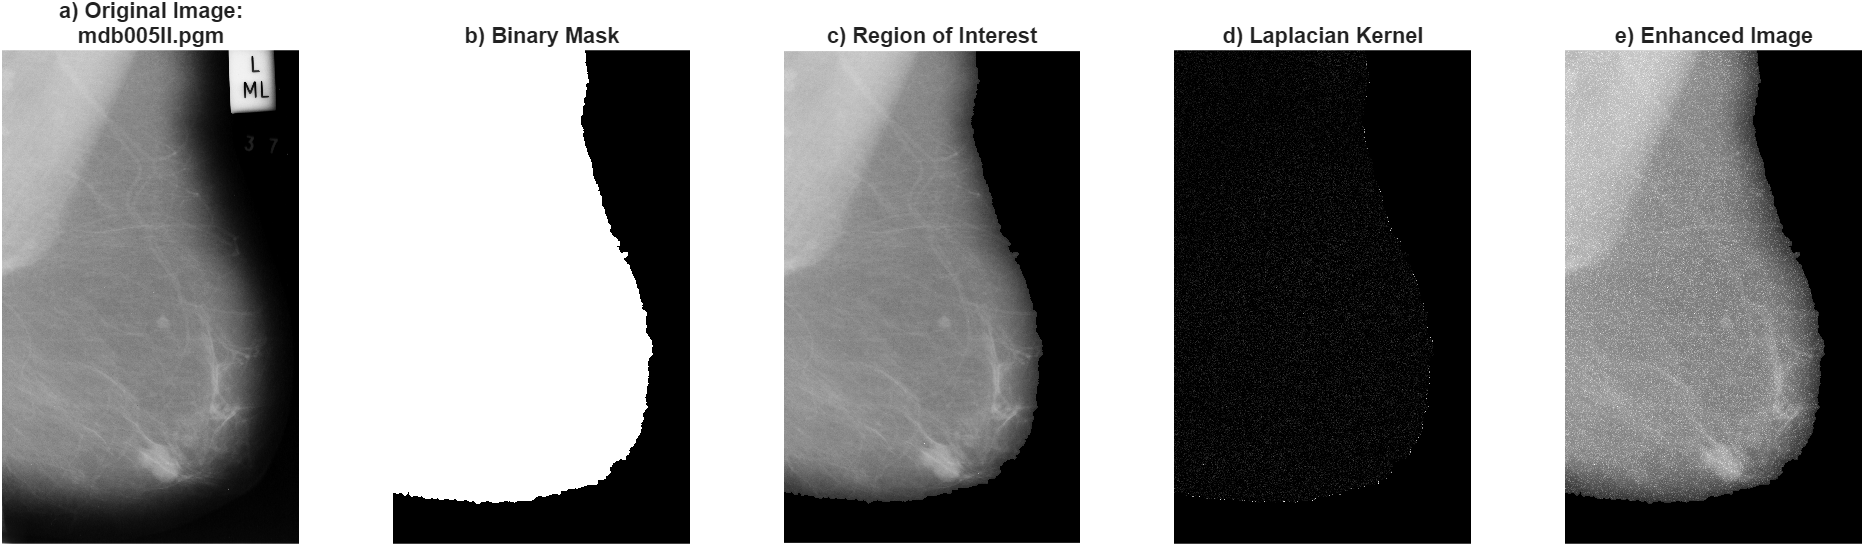
\includegraphics[width=0.9\textwidth]{./images/preprocessing.png}
\caption{Image enhancement pipeline: 
    a) Original mammogram image, 
    b) Binary mask isolating breast tissue, 
    c) Region of interest (ROI) extracted and refined, 
    d) Edge map generated using Laplacian kernel, 
    e) Final enhanced image with improved contrast and detail.
} \label{preprocessing-pipeline}
\end{figure}

\subsection{\ac{MedSAM} for Pectoral Muscle Segmentation}
\label{sec:zsl-with-medsam}
\Ac{ZSL} is a modern \ac{ML} paradigm in which a foundational model is
used to make predictions on data from classes or domains that were not
present in its training set without further training. These models are
generally transformer-based and rely on pre-training on a large
dataset.

Unlike traditional supervised learning, which requires labeled
examples for every target class, \ac{ZSL} enables generalization to
unseen categories by leveraging auxiliary information, such as
semantic attributes, textual descriptions, or embeddings from
pre-trained models. 

As previously discussed in Section~\ref{sec:found-models-image}, foundational
models such as \ac{SAM} and \ac{MedSAM} are capable of strong
zero-shot predictions on novel data. However, they require a visual
prompt to be supplied by the user. Consequently, using \ac{MedSAM} to
segment medical images introduces a \ac{HITL} component into the
process.

This research addresses two core research questions: (1) whether
foundational models such as \ac{MedSAM} can achieve accurate
segmentation in a \ac{ZSL} setting with \ac{HITL} prompting, and (2)
to benchmark the specific performance of \ac{MedSAM} under these
conditions.

\subsubsection{Experimental Design and Dataset}
To evaluate \ac{MedSAM}'s \ac{ZSL} performance, a ground-truth dataset
was constructed from the public \ac{MIAS} database. A sample of 170
mammograms was randomly selected, providing a 95\% confidence level
with a 5\% margin of error for statistical representativeness of the
dataset. This sample size ensures a robust evaluation while
maintaining a focus on the \ac{ZSL} scenario where extensive annotated
data is unavailable for training.

These sample images were distributed among five independent researchers
that manually labeled the pectoral muscle using \texttt{MATLAB Medical
  Image Labeler}. The Ground Truth Annotation Protocol consisted of:

% \subsubsection{Ground Truth Annotation Protocol}

\begin{itemize}
    \item \textbf{Manual Delineation:} Each annotator manually traced
      the pectoral muscle boundary using either polygon or Superpixel
      tools to ensure the annotated boundaries adhered to natural
      image textures.
    \item \textbf{Morphological Post-processing:} Standard
      morphological operations (dilation and erosion) were applied to
      smooth the masks, removing and filling small holes.
\end{itemize}

The final output for each image included binary masks for the
pectoral muscle and the glandular tissue, and a clean mammogram with
the pectoral muscle and background noise removed. 

\subsubsection{Zero-Shot Segmentation with \ac{MedSAM}}
\label{sec:medsam-methodology}
The core \ac{ZSL} experiment was conducted using the \ac{MedSAM} model
without any task-specific fine-tuning. For each test image, the model
was provided with a visual prompt over the preprocessed image. In
accordance with the \ac{HITL} paradigm central to the first research
question, this prompt was defined as a bounding box manually
delineated around the pectoral muscle region by a human operator. This
approach simulates a realistic clinical scenario requiring minimal
interaction. The operator was permitted to adjust the bounding box
dimensions to optimize the visual outcome. In all cases, the initial
anchor point for the bounding box was placed at the superior edge
where the muscle originates. \ac{MedSAM} generated the segmentation
mask based exclusively on this prompt and its pre-trained weights,
without employing any post-processing techniques such as dilation or
erosion. Figure~\ref{fig:ground_truth_example} presents an illustrative
example, comparing the manually annotated Ground Truth for case
\texttt{mdb048rm} with the \ac{ZSL} prediction generated by
\ac{MedSAM}.
% [[./images/ManualMask_vs_MedSAM_1.png]]
% [[./images/ManualMask_vs_MedSAM_2.png]]
% [[./images/ManualMask_vs_MedSAM_3.png]]
\begin{figure}[htbp]
    \centering
    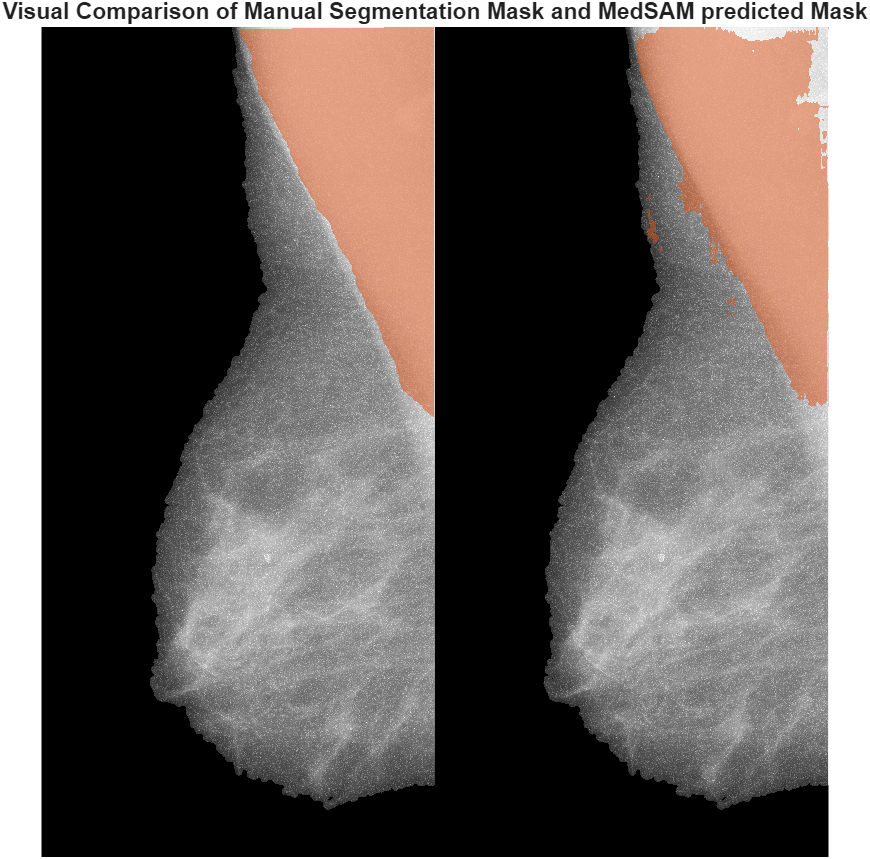
\includegraphics[scale=0.45]{./images/ManualMask_vs_MedSAM_3.png}
    \caption{Manually annotated Ground Truth for the pectoral muscle
      (left) and \ac{MedSAM}'s predicted mask (right) for \textrm{mdb048rm}.}
    \label{fig:ground_truth_example}
\end{figure}

\subsection{Recursive Otsu Threshold Algorithm for Mammogram Segmentation}
\label{sec:iter-otsu-algorithm}

The presence of the pectoral muscle in mammograms, especially in
\ac{MLO} views, represents a critical challenge for \ac{CADx} and
\ac{CADe} systems due to its intensity similarity to glandular
tissue. To address this issue,this study proposes a recursive,
multi-level application of Otsu's thresholding algorithm. The
challenge for a fully automated system is to detect the side
(left/right) of the breast in the mammogram and remove the pectoral
muscle from the correct location with precision. Our approach
determines whether the breast is left or right, generates a binary
mask for the pectoral muscle with user assistance, and combines the
tissue mask with the muscle-removed mask to produce the final image
without the pectoral muscle.
% the following image could be referenced when talking about the
% creation of the binary masks of pectoral muscel
% \begin{figure} 
% \centering
% \includegraphics[width=0.5\textwidth]{images/creationGT2.png}
% \caption{Interactive object segmentation is performed within user-defined ROIs using SAM, which employs deep learning and visual prompts to generate accurate binary masks. The first column shows the name of the image, the second shows the original image, and the third shows the overlay of the enhanced image without artifacts and the mask generated, using Matlab toolboxes} \label{fig7}
% \end{figure}

The objective of this method is to segment an image into multiple
intensity classes using recursive Otsu thresholding. The Otsu
thresholding method was originally proposed to segment images using a
single threshold that maximizes the between-class
variance~\cite{otsu1979}. However, many applications require
partitioning an image into more than two intensity regions, leading to
the development of multilevel
extensions~\cite{bioengineering11101034}. Among these, hierarchical or
recursive approaches apply the Otsu criterion iteratively to pixel
subsets to obtain adaptive multiple thresholds. This procedure, known
as recursive Otsu thresholding, has been successfully used in domains
such as medical image analysis and remote sensing due to its
simplicity and effectiveness in handling multimodal histograms.

The proposed algorithm begins by normalizing the raw input mammogram,
denoted as \( I_{\text{raw}} \), to a standard intensity range of
\([0, 1]\):

% \[
% I_0 = \frac{I_{\text{raw}} - \min(I_{\text{raw}})}{\max(I_{\text{raw}}) - \min(I_{\text{raw}})}.
% \]

\begin{equation}
I_0 = \frac{I_{\text{raw}} - \min(I_{\text{raw}})}{\max(I_{\text{raw}}) - \min(I_{\text{raw}})}
\label{eq:normalization}
\end{equation}

A global threshold, \( T_1 \), is first computed by applying Otsu's
method to the normalized image \( I_0 \). This algorithm selects the
threshold that maximizes the between-class variance, defined as:
% \[
% \sigma_B^2(T) = \omega_0(T)\,\omega_1(T)\,[\mu_0(T) - \mu_1(T)]^2,
% \]
\begin{equation}
\sigma_B^2(T) = \omega_0(T)\,\omega_1(T)\,[\mu_0(T) - \mu_1(T)]^2,
\label{eq:between_class_var}
\end{equation}
where \( \omega_0, \omega_1 \) and \( \mu_0, \mu_1 \) represent the
class probabilities and mean intensities for the foreground and
background classes, respectively. This initial step partitions the
image into two primary regions: a low-intensity region where
\( I_0 < T_1 \) and a high-intensity region where
\( I_0 \geq T_1 \).

To achieve a more granular segmentation for the  mammographic
tissue, Otsu's method is applied recursively within
each of these two regions. This yields two secondary thresholds:

% \[
% T_{\text{low}} = \text{Otsu}(I_0 \mid I_0 < T_1), \quad T_{\text{high}} = \text{Otsu}(I_0 \mid I_0 \geq T_1).
% \]

\begin{equation}
T_{\text{low}} = \text{Otsu}(I_0 \mid I_0 < T_1), \quad T_{\text{high}} = \text{Otsu}(I_0 \mid I_0 \geq T_1).
\label{eq:secondary_thresholds}
\end{equation}
A practical consideration is addressed for edge cases: if a subset
contains no pixels (e.g., an empty histogram), default threshold
values are assigned as \( T_{\text{low}} \approx T_1/2 \) and
\( T_{\text{high}} \approx (1+T_1)/2 \) to ensure robustness.

The final segmentation divides the mammogram into four distinct tissue
classes based on intensity, defined as follows:
% \[
% \begin{aligned}
% \text{Class 1: } & I_0 < T_{\text{low}}, \\
% \text{Class 2: } & T_{\text{low}} \leq I_0 < T_1, \\
% \text{Class 3: } & T_1 \leq I_0 < T_{\text{high}}, \\
% \text{Class 4: } & I_0 \geq T_{\text{high}}.
% \end{aligned}
% \]

\begin{equation}
\begin{aligned}
\text{Class 1: } & I_0 < T_{\text{low}}, \\
\text{Class 2: } & T_{\text{low}} \leq I_0 < T_1, \\
\text{Class 3: } & T_1 \leq I_0 < T_{\text{high}}, \\
\text{Class 4: } & I_0 \geq T_{\text{high}}.
\end{aligned}
\label{eq:final_classes}
\end{equation}
This recursive four-class segmentation procedure provides a foundational label
map that effectively differentiates between various density regions
within the \ac{MG}, which is a critical precursor for subsequent
analysis stages in the \ac{CADx}/\ac{CADe}
pipeline. Figure~\ref{fig:SegmentationMap} shows the segmentation map obtained
by applying our proposed methodology to the \texttt{mdb028rl} mammogram
directly, without preprocessing.

  \begin{figure}[ht]
    \centering
    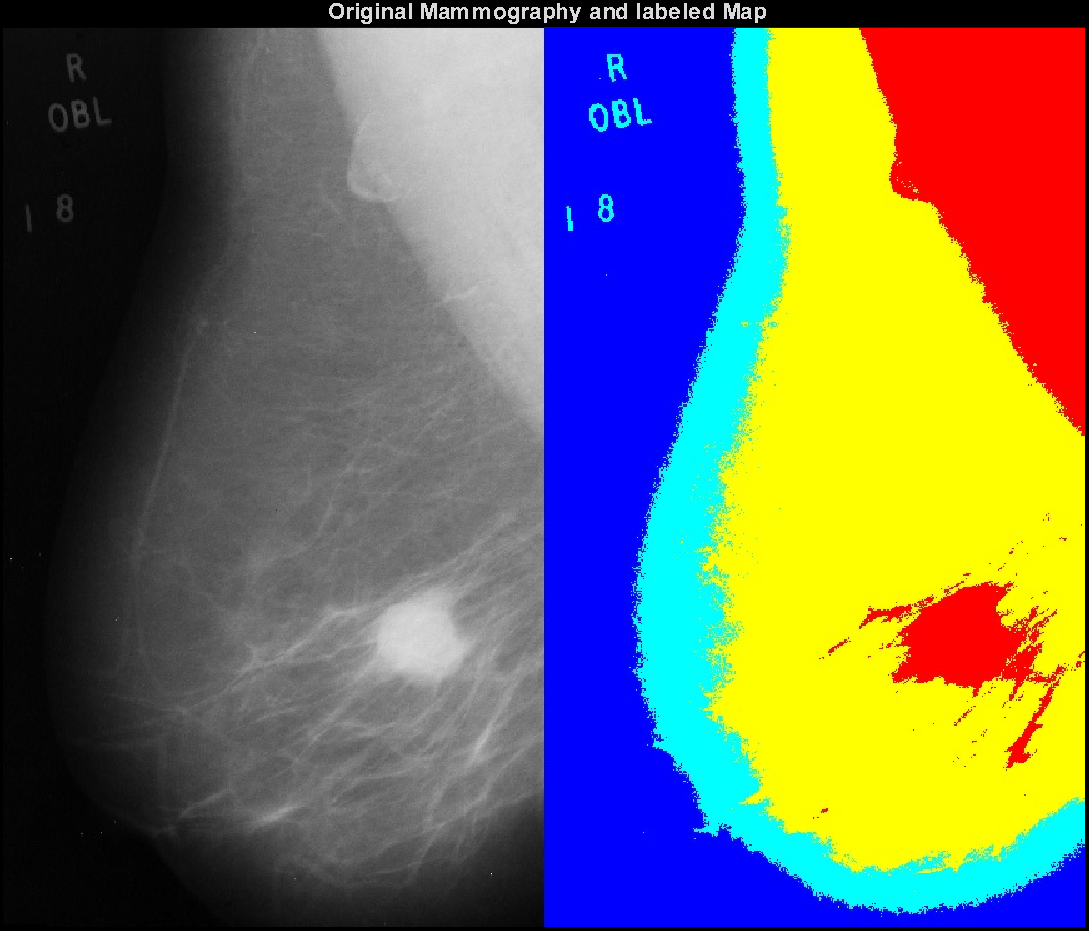
\includegraphics[scale=.45]{./images/pectoralMuscleProblem.pdf} %./presentation/figures_ppt/pectoralMuscleProblem.pdf
    \caption{\label{fig:SegmentationMap}Segmentation Map for
      \texttt{mdb028rl} using the recursive application of Otsu. The
      removal of the pectoral muscle allows the detection of
      suspicious masses}
  \end{figure}
\newpage
  
\section{Experimental Results}
\label{sec:experimental-results}
In this Section we address the performance of \ac{MedSAM} for \ac{ZSL}
segmentation of the pectoral muscle, using a labeled Ground Truth
dataset of our own, and of the proposed Recursive Otsu
approach for segmentation of masses in a mammogram. The latter
evaluation was carried out visually through the application of the
approach to samples of the \ac{MIAS} dataset presenting benign and
malignant masses.

The performance of the \ac{ZSL} approach was quantified by comparing
the masks generated by \ac{MedSAM} against the manual ground
truth. Standard segmentation metrics were computed, including
\ac{DICE}, \ac{IoU}, Precision and Recall, to assess spatial overlap
accuracy. This quantitative analysis directly addresses the second
research question regarding \ac{MedSAM}'s performance under \ac{ZSL}
conditions.

\subsection{Segmentation Performance Metrics}
\label{sec:segm-perf-metrics}
In binary segmentation, the \ac{DICE} coefficient and the
F\textsubscript{1}-score are algebraically
equivalent~\cite{Shen2018}. To quantitatively evaluate the performance
of the proposed methodology, we employ the following metrics, whose
mathematical definitions are provided in
Table~\ref{tab:segmentation_metrics}:
\begin{itemize}
\item \textbf{\ac{DICE}}: Defined by Eq.~\eqref{eq:dice}, measures the ratio of
  the correctly predicted positive pixels over the number of positive
  areas in both the Ground Truth and the prediction mask, considering
  the false positive rate in the calculations alongside false
  negatives. It has a range of [0,1], and a higher value indicates
  better performance\cite{Yao2023}.
\item \textbf{\ac{IoU}}: Also known as Jaccard Similarity coefficient, and
  defined in Eq.~\eqref{eq:iou}, quantifies the spatial overlap
  between a predicted segmentation mask and the corresponding ground
  truth mask (i.e. the size of the intersection divided by the size of
  the union of two label sets)~\cite{4781564,Yao2023}.
\item \textbf{Precision}: Measures the accuracy of positive predictions. In
  segmentation, it quantifies what proportion of the predicted
  foreground pixels are actually part of the true
  object. A closer value to 1 describes a higher precision and a more
  desired performance~\cite{Yao2023}. Eq.~\eqref{eq:precision} defines
  it mathematically.
\item \textbf{Recall}: Also known as Sensitivity, measures the completeness of
  detection. It quantifies what proportion of the actual foreground
  pixels are correctly identified by the model (i.e. the ratio of true
  positive samples to the total actual positive
  samples)~\cite{Yao2023}. Recall is defined by Eq.~\eqref{eq:recall}
  in Table~\ref{tab:segmentation_metrics}.
\end{itemize}

\begin{table}[h]
\centering
\caption{Common segmentation evaluation metrics. TP, FP, FN, and TN denote true positives, false positives, false negatives, and true negatives, respectively.}
\label{tab:segmentation_metrics}
\begin{tabular}{p{0.3\textwidth} p{0.6\textwidth}}
\toprule
\textbf{Metric} & \textbf{Equation}  \\
\midrule
Dice Similarity Coefficient (DSC) & 
\begin{equation}
\text{DSC} = \frac{2 \times \text{TP}}{2 \times \text{TP} + \text{FP} + \text{FN}}
\label{eq:dice}
\end{equation}  \\
\addlinespace
Intersection over Union (IoU) / Jaccard Index & 
\begin{equation}
\text{IoU} = \frac{\text{TP}}{\text{TP} + \text{FP} + \text{FN}}
\label{eq:iou}
\end{equation}  \\
\addlinespace
Precision (Positive Predictive Value) & 
\begin{equation}
\text{Precision} = \frac{\text{TP}}{\text{TP} + \text{FP}}
\label{eq:precision}
\end{equation}  \\
\addlinespace
Recall (Sensitivity) & 
\begin{equation}
\text{Recall} = \frac{\text{TP}}{\text{TP} + \text{FN}}
\label{eq:recall}
\end{equation}  \\
\bottomrule
\end{tabular}
\end{table}

\subsection{\ac{MedSAM} Experimental Results}
\label{sec:medsam-exper-results}
To assess the performance of \ac{MedSAM} for pectoral muscle
segmentation in \ac{MG} using \ac{ZSL} with \ac{HITL}, a comparison
was established between the predicted masks generated by the proposed
methodology (described in Section~\ref{sec:medsam-methodology}) and
the Ground Truth annotations in our labeled dataset. The results for
the metrics \ac{DICE}, \ac{IoU}, Precision, and Recall are presented
in Table~\ref{tab:medsam-results}. A total of 168 samples were used
for this evaluation, as two samples were discarded after the
preprocessing step due to the loss of the whole pectoral muscle
region. \ac{MedSAM} achieved a \ac{DICE} score of
\(0.86531 \pm 0.14039\) and an \ac{IoU} of \(0.78329 \pm
0.17118\). The maximum and minimum values for each metric correspond
to the best and worst performance of \ac{MedSAM}. For example,
\ac{MedSAM} attained the highest \ac{DICE} score of \(0.988\) for
image index 111 (i.e. \texttt{mdb160rl}), a median score of \(0.909\)
for image index 138 (\texttt{mdb247ll}), and the lowest score for
image index 43 (\texttt{mdb068rl}). These comparisons are presented in
Figure~\ref{fig:MedSamDiceScoreCompare}. Likewise,
Figure~\ref{fig:boxplot-summary} presents a boxplot summary of the
performance of \ac{MedSAM} in pectoral muscle segmentation task.

\begin{table}[h]
  \centering
  \caption{Quantitative evaluation results for \ac{MedSAM}}
  \label{tab:medsam-results}
  \begin{tabular}{lcccc}
    \hline
    \textbf{Metric} & \textbf{Mean $\pm$ Std} &
                                                \textbf{Median} & \textbf{Min} & \textbf{Max} \\
    \hline
    \ac{DICE}      & 0.86531 $\pm$ 0.14039 & 0.90895 & 0.15112  & 0.98791
    \\
    \ac{IoU}       & 0.78329 $\pm$ 0.17118 & 0.83310 & 0.08174  & 0.97611
    \\
    Precision & 0.92517 $\pm$ 0.14076 & 0.98206 & 0.08738  & 1.00000
    \\
    Recall    & 0.82970 $\pm$ 0.15068 & 0.87316 & 0.13349  & 0.99039
    \\
    \hline
    \end{tabular}
 \end{table}

 
 \begin{figure}[ht]
   \centering
   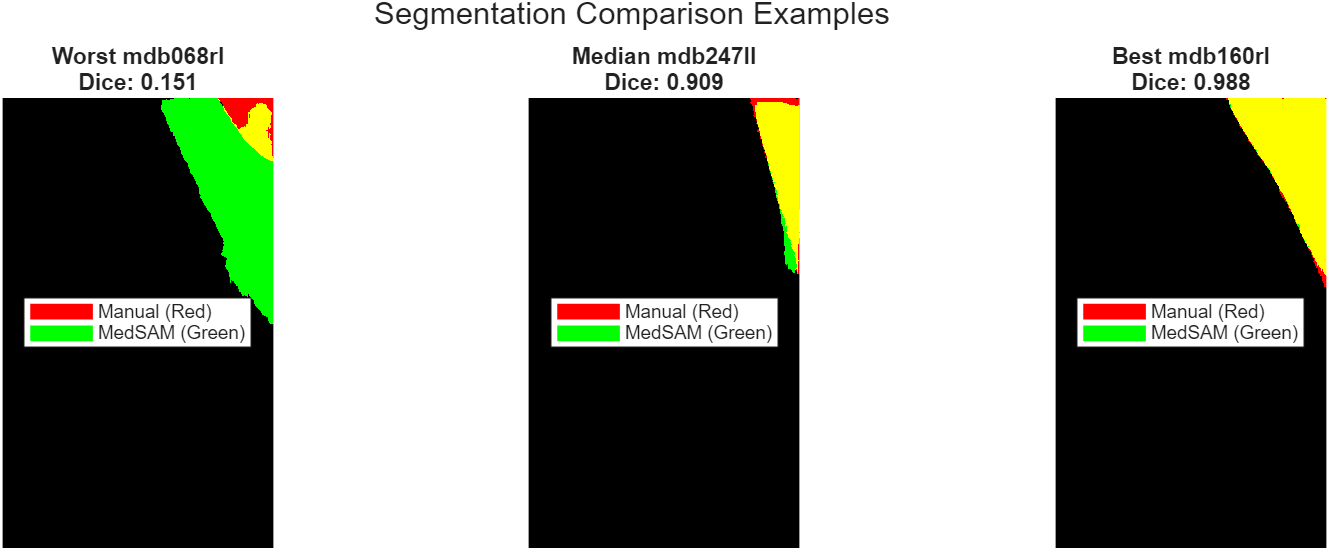
\includegraphics[width=\textwidth]{./images/SegmentationComparisonExamples_withLegend_vertical.png} %./presentation/figures_ppt/SegmentationComparisonExamples_withLegend.png
   \caption{Representative segmentation results of MedSAM showing
     worst (Image 43, \texttt{mdb068rl}), median (Image 138,
     \texttt{mdb247ll}), and best (Image 111, \texttt{mdb160rl}) cases
     with \ac{DICE} scores of 0.151, 0.909, and 0.988, respectively.}
   \label{fig:MedSamDiceScoreCompare}
 \end{figure}

\begin{figure}[ht]
  \centering
  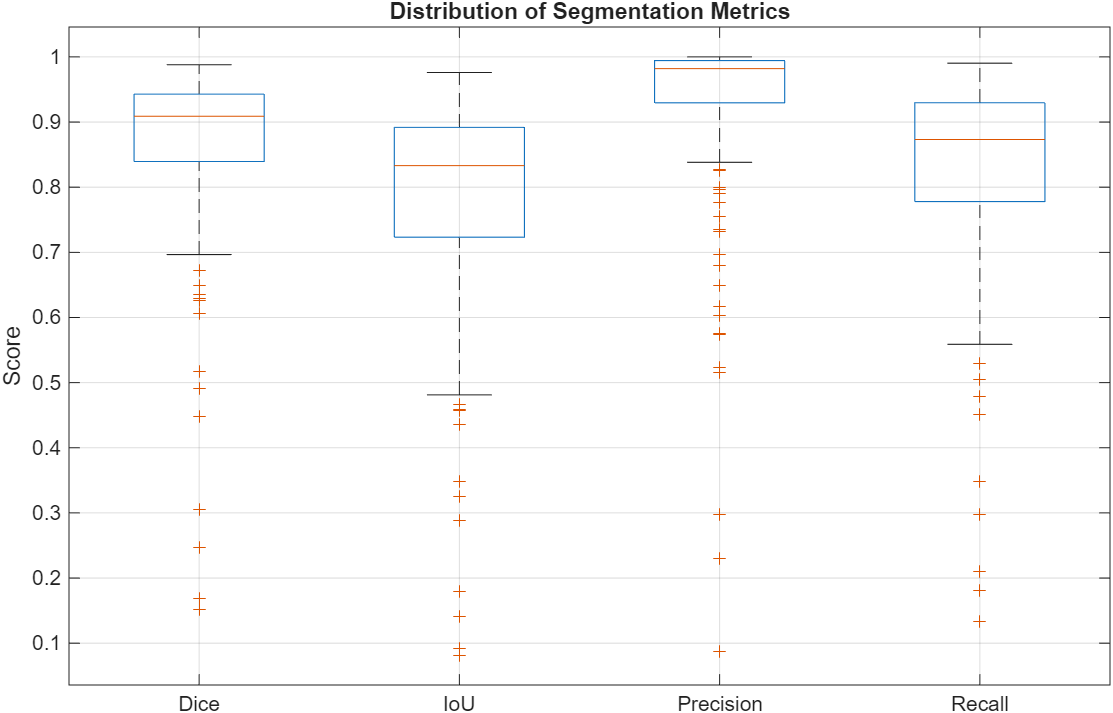
\includegraphics[width=\textwidth]{./images/SegmentationMetricsPerformance.png} %./presentation/figures_ppt/SegmentationMetricsPerformance.png
      \caption{Boxplot distribution of \ac{MedSAM}’s segmentation metrics
        for pectoral muscle detection using \ac{ZSL},
        showing variability across \ac{DICE}, \ac{IoU}, Precision, and Recall
        scores.}
      \label{fig:boxplot-summary}
      
\end{figure}
\newpage
\subsection{Qualitative validation of Recursive Otsu Threshold
  Algorithm}
\label{sec:qual-valid-recursive-otsu}

Visual validation was performed by overlaying the Ground Truth masks
with the proposed  segmentation masks from the recursive Otsu
Algorithm to assess their alignment and accuracy. By superimposing
these masks over the original images, visual inspection enabled the
evaluation of their spatial alignment, boundary accuracy, and overall
consistency, complementing the quantitative metrics

To evaluate the performance of the recursive thresholding approach for
mass detection, the mass region of the MIAS dataset was delineated
based on the information available in \texttt{Info.txt}. The script
extracts the Ground Truth information, including the lesion
coordinates and radio. Then, circular ROIs are drawn to approximate
the location and size of the lesions. This circular approximation is
suitable for general mass detection (e.g., CIRC, SPIC), but does not
represent the exact lesion contours. This was done to visually assess
the accuracy of the mass segmentation obtained with our
approach. Figure~\ref{fig:segmentation-pipeline-otsu} shows that the
ROI segmentation fits the automatically outlined circle.


% %%%%%%%%%%%%%%%%%%%% COLOCAR LA FIG 8 MEJORADA SOBRE LA LOCALIZACION
% DE LAS MASAS %%%%%%%%%%%%%%%%%%%%

\begin{figure}
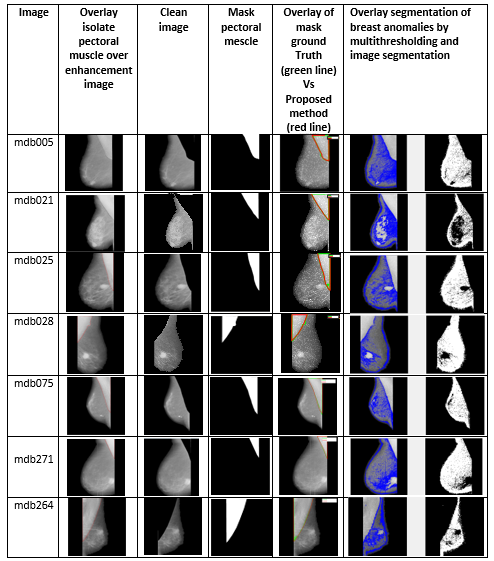
\includegraphics[width=\textwidth]{images/metodos.png}
\caption{Results of the proposed preprocessing and segmentation pipeline on representative mammographic images. From left to right: i) overlay of the isolated pectoral muscle on the enhanced image, ii) clean mammogram with background and muscle removed, iii) binary mask of the pectoral muscle, iv) comparison between ground-truth mask (green) and the proposed method (red), and (v) segmentation of breast anomalies obtained through multi-thresholding} \label{fig:segmentation-pipeline-otsu}
\end{figure}


% , as explained in Stage 3 (see Figures 6 and 8). It is
% clear that the ROI segmentation fits the automatically outlined
% circle.

\section{Discussion and Conclusion}
\label{sec:discussion-conclusion}

% \subsection{Summary of Contributions}
% [Briefly restate your main contributions]

\subsection{Discussion of Results}
Our investigation demonstrates that \ac{ZSL} with a foundation model,
specifically \ac{MedSAM}, can effectively aid in pectoral muscle
segmentation in mammograms, achieving a \ac{DICE} score near 0.90
without requiring further training. This indicates the strong
potential of foundation models to assist in labeling operations for
medical imaging data, thereby reducing the annotation burden. However,
these pseudo-segmentation masks cannot fully substitute for
radiologist-delineated Ground Truth. Expert annotations remain the
gold standard for clinical validation, as they incorporate contextual
knowledge and interpretative criteria beyond pixel-level delineation.

Concurrently, traditional image processing approaches, such as the
recursive Otsu's method proposed in this research, remain relevant for
segmentation tasks. A key advantage of this method is its independence
from \ac{MG} orientation and its significantly lower computational
cost compared to Transformer-based models like \ac{MedSAM}. However,
the recursive Otsu method necessitates the precise removal of the
pectoral muscle to facilitate subsequent mass detection. This step can
be readily integrated into the preprocessing pipeline of a
\ac{CADx}/\ac{CADe} system.

% This limitation can be addressed by developing a hybrid
% approach, for instance, by using a foundation model to guide the
% separation or by implementing a rule-based filter based on the
% calculated size and location of the segmented areas.

\subsection{Limitations}
The current study has several limitations that must be
acknowledged. First, the experimental validation was conducted on a
subset of the \ac{MIAS} dataset. The generalizability of our findings
needs to be confirmed on the complete dataset and other public
mammography repositories. Second, the Ground Truth annotations used
for evaluation were provided by individual researchers. Each
researcher worked with an independent set of samples. In order to
reduce potential labeling bias, it is recommended to implement a
consensus labeling set up. Third, the integration of \ac{HITL}
mechanisms for prompt refinement requires further investigation to
quantify and control for human biases introduced in the interactive
labeling process.

Finally, this study has not explored the performance of \ac{MedSAM}
through model fine-tuning. It should be noted, however, that
fine-tuning such models can lead to catastrophic forgetting, wherein
performance on the specific target task improves at the expense of the
model's generalization capabilities for its original source tasks.

% \subsection{Future Work}
% [Propose specific directions for extending this research]

\subsection{Conclusion}
This work explores both traditional and modern approaches for
mammogram segmentation. Despite the current trend in research toward
\ac{DL} for image segmentation in the medical domain, it is noteworthy
that traditional approaches, such as the recursive use of the Otsu
thresholding algorithm, can still yield strong results for mammogram
segmentation. On the other hand, foundational models like \ac{MedSAM}
exhibit robust \ac{OOD} generalization capabilities. To the best of
our knowledge, this research is the first to evaluate the performance
of this model on the important task of pectoral muscle
segmentation. Based on our current results, \ac{MedSAM} can be
employed in medical labeling workflows to reduce the burden of manual
annotation by generating pseudo-masks. However, the inherent design of
\ac{SAM} models introduces an \ac{HITL} factor through the requirement
for visual prompts. Future research could aim to automate this process
by developing either hybrid models that integrate both approaches or
fine-tuned versions of existing models.

\section*{Data Availability}
The source code, experimental setups, and supplementary materials
supporting this study are openly available in the GitHub repository at
\url{https://github.com/LeninGF/Modern-and-Traditional-Techniques-in-Mammogram-Segmentation.git}.


\begin{credits}
\subsubsection{\ackname} The authors of the Escuela Politecnica Nacional gratefully acknowledge the support provided by the PTT-03-02 project. This work was made possible thanks to the resources provided by this project and the institution.

%A bold run-in heading in small font size at the end of the paper is
%used for general acknowledgments, for example: This study was funded
%by X (grant number Y).

\subsubsection{\discintname}
 The authors have no competing interests to declare that are
relevant to the content of this article.
\end{credits}
%
% ---- Bibliography ----
%
% BibTeX users should specify bibliography style 'splncs04'.
% References will then be sorted and formatted in the correct style.
%
% \bibliographystyle{splncs04}
% \bibliography{mybibliography}
%
\bibliographystyle{splncs04}
\bibliography{bibliography}



\end{document}

%%% Local Variables:
%%% mode: LaTeX
%%% TeX-master: t
%%% End:
